 %--------------------------------------------------------------------%
% Berkas utama template LaTeX.
% author Petra Barus, Peb Ruswono Aryan - Dionesius Agung (2020)
%--------------------------------------------------------------------%

\documentclass[12pt, a4paper, onecolumn, oneside, final]{report}

%-------------------------------------------------------------------%
%
% Konfigurasi dokumen LaTeX untuk laporan tesis IF ITB
%
% @author Petra Novandi
% updated by Dionesius Agung (2020)
%-------------------------------------------------------------------%
%
% Berkas asli berasal dari Steven Lolong
%
%-------------------------------------------------------------------%

\usepackage[top=3cm,bottom=3cm,left=4cm,right=3cm,a4paper]{geometry}

\usepackage[english]{babel}

\renewcommand{\baselinestretch}{1.5}


%%%%%%%%%%%%%%%%%%%%%%%%%%%%%%%
%  BIBLIOGRAPHY AND CITATION  %
%%%%%%%%%%%%%%%%%%%%%%%%%%%%%%%
% use package biblatex
\usepackage[backend=biber,
            bibstyle=authoryear,
            citestyle=authoryear,
            sorting=nyt,
            url=false,
            maxcitenames=2,
            maxnames=2,
            dashed=false,
            uniquename=init,
            giveninits=true]{biblatex}
\DeclareNameAlias{author}{family-given}

% Translate bibliography strings ke bahasa indonesia
%   (karena 'bahasa' belum di-support)
\DefineBibliographyStrings{english}{%
  bibliography = {Daftar Pustaka},
  references = {Referensi},
  and = {\&},
  techreport = {Dok. teknis},
  phdthesis = {Disertasi doktoral\adddot},
  andothers = {dkk\adddot}
}

% Field berikut tidak ditulis di daftar pustaka
\AtEveryBibitem{\clearfield{issn}}
\AtEveryBibitem{\clearfield{isbn}}
\AtEveryBibitem{\clearfield{month}}
\AtEveryBibitem{\clearfield{doi}}

% Format entri daftar pustaka

%% Beri titik setelah judul
\DeclareFieldFormat
[article,inbook,incollection,inproceedings,
patent,unpublished,misc]
{title}{#1\isdot}

%% Judul buku ditulis italic
\DeclareFieldFormat
[thesis]
{title}{\emph{#1}\isdot}

%% Hilangkan kata "Dalam:" di antara judul artikel dan judul jurnal
\renewbibmacro{in:}{}

%% Format penulisan volume dan nomor pada jurnal: vol(num) e.g. 5(1)
\renewbibmacro*{volume+number+eid}{%
	\printfield{volume}%
	\printfield{number}%
	\setunit{\addcomma\space}%
	\printfield{eid}}
\DeclareFieldFormat[article]{number}{\mkbibparens{#1}}

% Format citation
\renewcommand*{\nameyeardelim}{\addcomma\space}

% Setting spasi di halaman daftar pustaka
\setlength\bibitemsep{0.5\baselineskip}


%%%%%%%%%%%%%%
%  PACKAGES  %
%%%%%%%%%%%%%%
\usepackage[utf8]{inputenc}
\usepackage{csquotes}
\usepackage{bookmark}
\usepackage{graphicx}
\usepackage{titling}
\usepackage{blindtext}
\usepackage{sectsty}
\usepackage{chngcntr}
\usepackage{etoolbox}
\usepackage{hyperref}       % Package untuk link di daftar isi.
\usepackage{titlesec}       % Package Format judul
\usepackage{parskip}
\usepackage{pdflscape}
\usepackage{afterpage}
\usepackage{ltablex}
\usepackage{booktabs}
\usepackage{tabularx}
\usepackage{multirow}
\usepackage[table,xcdraw]{xcolor}


%%%%%%%%%%%%%%$$%%%%%%%%%
%  CHAPTER AND SECTION  %
%%%%%%%%%%%%%%%%$$%%%%%%%
% Format judul bab
\chapterfont{\centering \large}
\titleformat{\chapter}[display]
  {\large\centering\bfseries}
  {\chaptertitlename\ \thechapter}{0em}
    {\large\bfseries\MakeUppercase}
\titlespacing*{\chapter}
	{0pt}
	{-1.5\baselineskip}
	{1.5\baselineskip}

% Format judul section (dan sub(sub)section)
\titleformat*{\section}{\bfseries\normalsize}
\titleformat*{\subsection}{\bfseries\normalsize}
\titleformat*{\subsubsection}{\bfseries\normalsize}
\titlespacing*{\section}{0pt}{1ex}{0pt}
\titlespacing*{\subsection}{0pt}{1ex}{0pt}
\titlespacing*{\subsubsection}{0pt}{1ex}{0pt}

% Kedalaman hierarki section (paling dalam subsubsection)
\setcounter{secnumdepth}{3}

\hbadness=99999
\vbadness=99999

%%%%%%%%%%%%%%%%%%%%%%%%%%%%%%%%%%%%%%%%%%%%%%%%%%
%  TABLE OF CONTENTS, LISTS OF FIGURES & TABLES  %
%%%%%%%%%%%%%%%%%%%%%%%%%%%%%%%%%%%%%%%%%%%%%%%%%%
\usepackage[titles]{tocloft}
% \usepackage[titletoc]{appendix}
\usepackage{tocbibind}

% Kedalaman hierarki maksimum ToC
% (yang masuk ToC hanya sampai subsection: I.1.1.)
\setcounter{tocdepth}{2}

% Hilangkan gap antar-bab di ToC
\setlength{\cftbeforechapskip}{0pt}

% Tambah kata "BAB" sebelum nomor bab di daftar isi
% TODO: still problematic when used with list of appendices (uncomment these 4 following lines to reproduce the problem)
\renewcommand{\cftchappresnum}{BAB~} % BAB before number in ToC
\newlength{\mylen} % a scratch length
\settowidth{\mylen}{\bfseries\cftchappresnum\cftchapaftersnum} % extra space
\addtolength{\cftchapnumwidth}{\mylen} % add the extra space

\renewcommand{\cftchapleader}{\cftdotfill{\cftdotsep}}

% Pisah daftar lampiran dari ToC
%%%
% \renewcommand{\appendixtocname}{Daftar Lampiran}

% \makeatletter
% \let\oldappendix\appendices

% \renewcommand{\appendices}{%
%   \clearpage
%   % From now, everything goes to the app file and not to the toc
%   \let\tf@toc\tf@app
%   \addtocontents{app}{\protect\setcounter{tocdepth}{1}}
%   \immediate\write\@auxout{%
%     \string\let\string\tf@toc\string\tf@app^^J
%   }
%   \oldappendix
% }%

\newcommand{\listofappendices}{%
  \begingroup
  \renewcommand{\contentsname}{\appendixtocname}
  \let\@oldstarttoc\@starttoc
  \def\@starttoc##1{\@oldstarttoc{app}}
  % Reusing the code for \tableofcontents with different
  %   \contentsname and different file handle app
  \tableofcontents
  \endgroup
}
\makeatother
%%%

% Hilangkan gap antara entri gambar & tabel antarbab di daftar tabel 
% dan daftar gambar (hanya terlihat kalau ada gambar/tabel di >1 bab)
\newcommand*{\noaddvspace}{\renewcommand*{\addvspace}[1]{}}
\addtocontents{lof}{\protect\noaddvspace}
\addtocontents{lot}{\protect\noaddvspace}


%%%%%%%%%%%%%%%%%%%%%%%%%%%%%%%%%%%%%%%%%
%  FLOATS: FIGURES, TABLES, ALGORITHMS  %
%%%%%%%%%%%%%%%%%%%%%%%%%%%%%%%%%%%%%%%%%
% Before:
% ---
% Counter untuk figure dan table.
% \counterwithin{figure}{section}
% \counterwithin{table}{section}
% ---
\renewcommand\dateenglish{%
 \def\today{\number\day\space\ifcase\month\or
    Januari\or Februari\or Maret\or April\or Mei\or Juni\or
    Juli\or Agustus\or September\or Oktober\or November\or
    Desember\fi
    \space\number\year}}
\def\thismonth{\ifcase\month\or
Januari\or Februari\or Maret\or April\or Mei\or Juni\or
Juli\or Agustus\or September\or Oktober\or November\or
Desember\fi
\space\number\year}

\usepackage[labelsep=period,
justification=justified,
format=hang,
figurename=Gambar,
tablename=Tabel]{caption}
\usepackage[labelformat=simple]{subcaption}
%% Hack subfigure cross-ref agar pakai tanda kurung
%%   e.g. Gambar II.2(a), bukan Gambar II.2a
%% (method recommended in subcaption package documentation)
\renewcommand\thesubfigure{(\alph{subfigure})}

% Counter untuk gambar dan tabel
\renewcommand*{\thefigure}{\thechapter.\arabic{figure}}
\renewcommand*{\thetable}{\thechapter.\arabic{table}}

% Jarak spasi antara float dengan teks utama
\captionsetup[figure]{belowskip=-1em}
% \captionsetup[subfigure]{belowskip=0pt}
\setlength{\textfloatsep}{2\baselineskip}
\setlength{\intextsep}{2\baselineskip}

% Spasi single di environment table
\AtBeginEnvironment{table}
  {\renewcommand{\baselinestretch}{1.0}}

% Avoid widow and orphan lines if possible
\widowpenalty500
\clubpenalty10000

% Hyphenation penalty
\hyphenpenalty=10000
\tolerance=1
\sloppy

\usepackage[chapter]{algorithm}
\usepackage{algpseudocode}
% Rename "Algorithm" into "Algoritma"
\makeatletter
\renewcommand*{\ALG@name}{Algoritma}
\newcommand{\algorithmname}{\ALG@name}
\makeatother


%%%%%%%%%%%%%%%%%%%%%%%%%
%  MATHS AND EQUATIONS  %
%%%%%%%%%%%%%%%%%%%%%%%%%
\usepackage{amsmath}
\usepackage{amsfonts}
\usepackage{mathtools}

% Counter untuk equation
\renewcommand*{\theequation}{\thechapter.\arabic{equation}}

% Allow page breaks on long equations
\allowdisplaybreaks[1-4]

\makeatletter
\makeatother

\addbibresource{references.bib}

\begin{document}
%Basic configuration
\title{Pelacakan Objek Dinamis menggunakan Pengukuran Banyak Agen dengan Latensi Komunikasi pada Robot Kontes Sepak Bola Beroda}
\date{\today}
\author{
    Bimo Adityarahman Wiraputra \\
    NIM: 13517004
}

\pagenumbering{roman}
\setcounter{page}{0}

\clearpage
\pagestyle{empty}

\newgeometry{top=3cm,bottom=3cm,left=3cm,right=3cm}

{\fontfamily{ptm}\selectfont%
    \begin{center}

        \smallskip

        \large{\bfseries \MakeUppercase{\thetitle}}
        \\[2\baselineskip]

        \large{\bfseries Laporan Tugas Akhir I}
        \\[\baselineskip]

        \normalsize{ \bfseries
            Disusun sebagai syarat kelulusan mata kuliah \\
            IF4091/Tugas Akhir I dan Seminar
        }
        \\[3\baselineskip]

        \normalsize{ \bfseries Oleh\\}
        \large{ \bfseries \MakeUppercase{\theauthor}}

        \vfill
        \begin{figure}[h]
            \centering
            
\includegraphics[height=3.5cm,keepaspectratio]{resources/cover-ganesha.jpg}
        \end{figure}
        \vfill

        \large{ \bfseries
            \uppercase{
                Program Studi Teknik Informatika \\
                Sekolah Teknik Elektro dan Informatika \\
                Institut Teknologi Bandung\\
            }
            \thismonth
        }

    \end{center}
}%

\restoregeometry
\clearpage

\clearpage
\pagestyle{empty}

\begin{center}

    \large{\bfseries \MakeUppercase{\thetitle}}
    \\[2\baselineskip]

    \large{\textbf{Laporan Tugas Akhir I}}
    \\[2\baselineskip]

    \normalsize{Oleh\\
    \MakeUppercase{\textbf{\theauthor}}\\
    \textbf{Program Studi Teknik Informatika} \\
    Sekolah Teknik Elektro dan Informatika \\
    Institut Teknologi Bandung}
    \\[4\baselineskip]


    \normalsize{Bandung, \today \\
    Mengetahui, \\[1\baselineskip]
    Pembimbing,\\[4\baselineskip]
    \underline{Dr. Judhi Santoso, M.Sc.}\\
    NIP. 196302041989031002}

\end{center}
\clearpage

% \input{chapters/statement}

\pagestyle{plain}

% \input{chapters/abstract-id}
% \input{chapters/forewords}

% Hacks to capitalize all chapter-level titles in ToC
\renewcommand*\contentsname{DAFTAR ISI}
% \renewcommand*\appendixtocname{DAFTAR LAMPIRAN}
\renewcommand*\listfigurename{DAFTAR GAMBAR}
\renewcommand*\listtablename{DAFTAR TABEL}
\renewcommand*\bibname{DAFTAR PUSTAKA}

% Lanjutan frontmatter
\tableofcontents
% \listofappendices
{%
    \let\oldnumberline\numberline%
    \renewcommand{\numberline}{\figurename~\oldnumberline}%
    \listoffigures%
}
{%
    \let\oldnumberline\numberline%
    \renewcommand{\numberline}{\tablename~\oldnumberline}%
    \listoftables%
}


%----------------------------------------------------------------%
% Konfigurasi Bab
%----------------------------------------------------------------%
%------------------------------------------------------%
% Hack: 2 baris berikut dipindah ke chapter-1.tex
%   previous method: nomor halaman sebelum BAB I jadi 0
%------------------------------------------------------%
% \pagenumbering{arabic}
% \setcounter{page}{0}
\renewcommand{\chaptername}{BAB}
\renewcommand{\thechapter}{\Roman{chapter}}
%----------------------------------------------------------------%

%----------------------------------------------------------------%
% Daftar Bab
%----------------------------------------------------------------%
\chapter{PENDAHULUAN}
\pagenumbering{arabic}
\setcounter{page}{1}

Bab ini memaparkan latar belakang yang mendasari penulisan tugas akhir ini; rumusan masalah, tujuan, dan batasan tugas akhir secara formal; sampai metodologi pengerjaan tugas akhir ini.

\section{Latar Belakang}

Studi di bidang robotika merupakan salah satu bidang riset dalam lingkup intelijensi buatan yang memiliki aplikasi yang sangat luas dalam kehidupan manusia. Perkembangan robotika telah memiliki dampak yang sangat besar dalam perkembangan zaman, terutama di bidang industri manufaktur dimana robot memungkinkan pekerjaan kompleks untuk dilakukan dengan volume tinggi. Secara umum, robotika telah maupun sangat berpotensi untuk membantu menciptakan peralatan otomatis yang dapat mengerjakan pekerjaan kompleks dengan akurasi, kecepatan, ketahanan, maupun tingkat keamanan yang lebih tinggi dibandingkan dengan manusia di berbagai bidang lainnya, seperti industri pertahanan, pertambangan, sampai industri kesehatan.

Dalam studi dan pengembangan robotika, peneliti mengkaji dan mempelajari bagaimana robot dapat direkayasa untuk menyelesaikan pekerjaan yang kompleks. Lingkup studi ini pun mencakup area yang luas, dari bagaimana robot dapat berinteraksi dengan manusia sampai bagaimana robot dapat berkoordinasi dengan banyak robot lainnya dalam menyelesaikan pekerjaannya. Sebagai sistem fisik siber, robot yang baik dapat melakukan persepsi dan membaca keadaan dunia dengan akurat, melakukan komputasi dan pengambilan keputusan tingkat tinggi, dan mengeksekusi suatu aksi dengan presisi.

Salah satu inisiatif untuk membangkitkan perkembangan di bidang robotika ini adalah liga pertandingan Robocup, yang merupakan liga pertandingan terbuka untuk tim pengembang dari universitas maupun organisasi lainnya untuk merekayasa robot-robot yang dapat ditandingkan antar tim. Diantara cabang liga yang ditandingkan dalam Robocup adalah kompetisi robot sepak bola beroda, dimana peserta mengembangkan tim robot-robot beroda yang harus berkoordinasi untuk mencetak gol di gawang lawan. Misi awal RoboCup saat didirikan adalah untuk mengumpulkan tim robot yang cukup maju untuk dapat mengalahkan tim manusia juara Piala Dunia pada tahun 2050. Inisiatif serupa juga ada di Indonesia dalam bentuk Kontes Robot Indonesia yang diselenggarakan oleh Kementrian Pendidikan dan Kebudayaan antar tim dari universitas-universitas Indonesia.

Dalam rekayasa robotika, pembuatan modul persepsi yang akurat merupakan hal yang penting karena bacaan \textit{world state} atau keadaan dunia merupakan masukan robot untuk melakukan pengambilan keputusan dan aksi, sehingga kualitas bacaan yang buruk dapat mengakibatkan pengambilan keputusan yang salah dan membahayakan keamanan robot itu sendiri, pengguna, maupun orang lain yang mungkin terlibat. Dalam konteks robot sepak bola beroda, pelacakan posisi robot sendiri (yang disebut juga lokalisasi), posisi robot lawan, maupun posisi bola merupakan informasi yang penting yang digunakan di banyak level dari pengambilan keputusan dan strategi tim sampai fungsionalitas dasar seperti mengejar, menggiring, mengoper, dan menembak bola.

Selain pengolahan data dari sensor yang dimiliki robot sendiri, pertukaran dan pengolahan data dari robot yang lain juga merupakan hal yang penting dalam pembacaan \textit{world state} untuk mendapatkan bacaan yang selengkap dan seakurat mungkin. Dalam kontes robot sepak bola, tidak terbacanya posisi suatu objek merupakan hal yang sering terjadi karena batasan jarak efektif sensor maupun halangan visual dari objek lain. Keterlambatan atau kegagalan penyampaian informasi dari suatu robot ke robot lain yang juga dapat terjadi karena inferensi jaringan terutama di tempat kontes yang memiliki banyak penonton mengharuskan representasi informasi yang dipertukarkan dan algoritma pengolahan informasi pada robot harus didesain dengan baik.

Telah terdapat banyak penelitian mengenai cara penggabungan bacaan keadaan dari banyak robot di dalam maupun luar konteks robot sepak bola beroda, dan ada beberapa studi modifikasi algoritma estimasi sensor dengan masukan data yang mungkin terlambat, akan tetapi masih sedikit penelitian yang membahas penggabungan bacaan keadaan dari banyak robot dalam konteks robot sepak bola beroda yang mempertimbangkan latensi di komunikasi.

Dalam tugas akhir ini, penulis meneliti dan menguji coba modul persepsi pembacaan \textit{world state} di lingkungan robot yang dikembangkan DAGOZILLA yang merupakan tim pengembang robot sepak bola beroda di ITB yang hendak mengikuti Kontes Robotika Indonesia dan RoboCup sebagai tempat yang tepat untuk dapat mengaplikasikan dan menguji coba modul tersebut di berbagai kondisi nyata di lapangan.

\section{Rumusan Masalah}

Masalah yang hendak diselesaikan pada tugas akhir ini adalah mengenai desain dan pembuatan algoritma persepsi \textit{world state} menggunakan pertukaran informasi banyak robot dengan latensi komunikasi, spesifik pada kasus pengembangan robot sepak bola beroda di tim DAGOZILLA ITB. Untuk menyelesaikan permasalahan tersebut, masalah dibagi menjadi beberapa submasalah:

\begin{enumerate}
    \item Bagaimana memproses data dari sensor robot itu sendiri?
    \item Bagaimana merepresentasi informasi yang akan dikirimkan ke robot lain?
    \item Bagaimana memproses informasi yang diterima dari robot lain yang mungkin terlambat karena latensi komunikasi?
\end{enumerate}

\section{Tujuan}

Tujuan dari tugas akhir ini terdiri dari beberapa poin:

\begin{enumerate}
    \item Mendapatkan algoritma yang baik untuk memproses data dari sensor robot sendiri
    \item Mendapatkan representasi yang baik untuk informasi yang akan dikirimkan ke robot lain
    \item Mendapatkan algoritma yang baik untuk memproses informasi dari robot lain yang mungkin terlambat
    \item Melakukan implementasi algoritma di lingkungan robot tim DAGOZILLA
\end{enumerate}

\section{Batasan Masalah}

Batasan masalah yang diambil untuk membatasi lingkup penelitian di tugas akhir ini adalah:

\begin{enumerate}
    \item \textit{World state} yang diestimasi mencakup posisi robot anggota tim dan lawan, dan posisi bola pada saat ini di lapangan
    \item Eksperimen dilakukan dengan simulasi dengan validasi menggunakan uji coba di lapangan menggunakan robot tim DAGOZILLA
    \item Jenis sensor yang digunakan dan frekuensi bacaan menyesuaikan konfigurasi robot tim DAGOZILLA
    \item Pemodelan \textit{error} di bacaan sensor dan latensi komunikasi disesuaikan sedekat mungkin dengan kondisi nyata di robot tim DAGOZILLA
\end{enumerate}

\section{Metodologi}

Pengerjaan tugas akhir dibagi menjadi beberapa tahapan:

\begin{enumerate}
    \item Pemodelan lingkungan dunia nyata

          Pada tahap ini, dimodelkan lingkungan dunia nyata tempat robot bekerja, termasuk distribusi \textit{error} dari sensor dan distribusi latensi dari komunikasi.

    \item Pembuatan lingkungan simulasi

          Pada tahap ini, dibuat lingkungan simulasi yang dapat disambungkan dengan lingkungan kode robot untuk melakukan pengujicobaan dengan profil \textit{error} dan latensi sesuai yang sudah didapat sebelumnya.

    \item Implementasi dan pengujicobaan algoritma pembanding

          Pada tahap ini, diimplementasi dan diuji coba algoritma-algoritma dari referensi sebagai pembanding untuk algoritma hipotesis yang akan dikembangkan.

    \item Desain dan implementasi algoritma hipotesis

          Pada tahap ini, dilakukan desain dan implementasi algoritma hipotesis di lingkungan robot agar dapat diujicobakan.

    \item Pengujicobaan dan analisis algoritma hipotesis

          Pada tahap ini, dilakukan uji coba dan analisis dari performa algoritma hipotesis berdasarkan tujuan tugas akhir dan perbandingannya dengan algoritma pembanding.
\end{enumerate}

\section{Jadwal Pelaksanaan Tugas Akhir}

Waktu pengerjaan tugas akhir ini dibagi berdasarkan diagram:

\clearpage% Flush earlier floats (otherwise order might not be correct)
\newgeometry{margin=2cm}
\begin{landscape}% Landscape page

    \begin{table}
        \setlength\tabcolsep{0pt}
        \caption{\textit{Gantt chart} Tugas Akhir 1} \label{tab:final-project-1}
        \addtocounter{table}{-1}
        \begin{tabularx}{\linewidth}{X *{18}{>{\centering\arraybackslash}m{15pt}}X}
            \toprule
            \multicolumn{1}{c}{}                                          &
            \multicolumn{5}{c}{Sept.}                                     &
            \multicolumn{4}{c}{Okt.}                                      &
            \multicolumn{4}{c}{Nov.}                                      &
            \multicolumn{5}{c}{Des.}                                      &
            \multicolumn{1}{c}{}                                                                                                     \\ \cmidrule{2-19}

            \multicolumn{1}{c}{\multirow{-2}{*}{Pekerjaan}}               &
            \multicolumn{1}{c}{1}                                         &
            \multicolumn{1}{c}{2}                                         &
            \multicolumn{1}{c}{3}                                         &
            \multicolumn{1}{c}{4}                                         &
            \multicolumn{1}{c}{5}                                         &
            \multicolumn{1}{c}{1}                                         &
            \multicolumn{1}{c}{2}                                         &
            \multicolumn{1}{c}{3}                                         &
            \multicolumn{1}{c}{4}                                         &
            \multicolumn{1}{c}{1}                                         &
            \multicolumn{1}{c}{2}                                         &
            \multicolumn{1}{c}{3}                                         &
            \multicolumn{1}{c}{4}                                         &
            \multicolumn{1}{c}{1}                                         &
            \multicolumn{1}{c}{2}                                         &
            \multicolumn{1}{c}{3}                                         &
            \multicolumn{1}{c}{4}                                         &
            \multicolumn{1}{c}{5}                                         &
            \multicolumn{1}{c}{\multirow{-2}{*}{Luaran}}                                                                             \\ \midrule

            \multicolumn{20}{l}{1. Studi Literatur}                                                                                  \\ \midrule
            Pengajuan topik dan dosen pembimbing                          &   &   &  &
            \cellcolor[HTML]{333333}                                      &   &   &  &   &   &   &   &   &   &  &   &   &  &   &     \\ \cmidrule{1-1}
            Studi literatur referensi topik                               &   &   &  &   &
            \cellcolor[HTML]{333333}{\color[HTML]{333333} }               &
            \cellcolor[HTML]{333333}{\color[HTML]{333333} }               &   &   &  &   &   &   &   &   &   &  &   &                \\ \cmidrule{1-1}
            Penulisan bab 2                                               &   &   &  &   &   &
            \cellcolor[HTML]{333333}{\color[HTML]{333333} }               &
            \cellcolor[HTML]{333333}{\color[HTML]{333333} }               &   &   &  &   &   &   &   &   &   &  &   &
            \multirow{-3}{=}{Draft Bab 2 Studi Literatur}                                                                            \\ \midrule

            \multicolumn{20}{l}{2. Lingkup, Rumusan Masalah, dan Metode}                                                             \\ \midrule
            Penentuan lingkup dan metode                                  &   &   &  &   &   &   &   &
            \cellcolor[HTML]{333333}{\color[HTML]{333333} }               &
            \cellcolor[HTML]{333333}{\color[HTML]{333333} }               &
            \cellcolor[HTML]{333333}{\color[HTML]{333333} }               &   &   &  &   &   &   &   &   &
            Draft Bab 1 Pendahuluan                                                                                                  \\ \midrule

            \multicolumn{20}{l}{3. Pemodelan, Analisis, dan Perancangan}                                                             \\ \midrule
            Pemodelan lingkungan dunia                                    &   &   &  &   &   &   &   &   &   &  &
            \cellcolor[HTML]{333333}{\color[HTML]{333333} }               &
            \cellcolor[HTML]{333333}{\color[HTML]{333333} }               &   &   &  &   &   &   &                                   \\ \cmidrule{1-1}
            Pemilihan algoritma pembanding dan desain algoritma hipotesis &   &   &  &   &   &   &   &   &   &  &   &
            \cellcolor[HTML]{333333}{\color[HTML]{333333} }               &
            \cellcolor[HTML]{333333}{\color[HTML]{333333} }               &   &   &  &   &   &
            \multirow{-2}{=}{Draft Bab 3 Analisis dan Perancangan}                                                                   \\ \cmidrule{1-1} \cmidrule{20-20}
            Pengumpulan Buku Tugas Akhir 1                                &   &   &  &   &   &   &   &   &   &  &   &   &  &
            \cellcolor[HTML]{333333}{\color[HTML]{333333} }               &   &   &  &   &
            Buku Tugas Akhir 1                                                                                                       \\ \cmidrule{1-1} \cmidrule{20-20}
            Seminar Tugas Akhir 1                                         &   &   &  &   &   &   &   &   &   &  &   &   &  &   &   &
            \cellcolor[HTML]{333333}{\color[HTML]{333333} }               &
            \cellcolor[HTML]{333333}{\color[HTML]{333333} }               &   &                                                      \\ \bottomrule
        \end{tabularx}
    \end{table}

    \pagebreak

    \begin{table}
        \setlength\tabcolsep{0pt}
        \caption{\textit{Gantt chart} Tugas Akhir 2} \label{tab:final-project-2}
        \addtocounter{table}{-1}
        \begin{tabularx}{\linewidth}{X *{26}{>{\centering\arraybackslash}m{12pt}}X}
            \toprule
            \multicolumn{1}{c}{}                            &
            \multicolumn{4}{c}{Jan.}                        &
            \multicolumn{4}{c}{Feb.}                        &
            \multicolumn{5}{c}{Mar.}                        &
            \multicolumn{4}{c}{Apr.}                        &
            \multicolumn{4}{c}{Mei}                         &
            \multicolumn{5}{c}{Juni}                        &
            \multicolumn{1}{c}{}                                                                                                              \\ \cmidrule{2-27}


            \multicolumn{1}{c}{\multirow{-2}{*}{Pekerjaan}} &
            \multicolumn{1}{c}{1}                           &
            \multicolumn{1}{c}{2}                           &
            \multicolumn{1}{c}{3}                           &
            \multicolumn{1}{c}{4}                           &
            \multicolumn{1}{c}{1}                           &
            \multicolumn{1}{c}{2}                           &
            \multicolumn{1}{c}{3}                           &
            \multicolumn{1}{c}{4}                           &
            \multicolumn{1}{c}{1}                           &
            \multicolumn{1}{c}{2}                           &
            \multicolumn{1}{c}{3}                           &
            \multicolumn{1}{c}{4}                           &
            \multicolumn{1}{c}{5}                           &
            \multicolumn{1}{c}{1}                           &
            \multicolumn{1}{c}{2}                           &
            \multicolumn{1}{c}{3}                           &
            \multicolumn{1}{c}{4}                           &
            \multicolumn{1}{c}{1}                           &
            \multicolumn{1}{c}{2}                           &
            \multicolumn{1}{c}{3}                           &
            \multicolumn{1}{c}{4}                           &
            \multicolumn{1}{c}{1}                           &
            \multicolumn{1}{c}{2}                           &
            \multicolumn{1}{c}{3}                           &
            \multicolumn{1}{c}{4}                           &
            \multicolumn{1}{c}{5}                           &
            \multicolumn{1}{c}{\multirow{-2}{*}{Luaran}}                                                                                      \\ \midrule

            \multicolumn{28}{l}{4. Implementasi dan Pengujian}                                                                                \\ \midrule
            Implementasi lingkungan simulasi                &   &  &
            \cellcolor[HTML]{333333}                        &
            \cellcolor[HTML]{333333}                        &
            \cellcolor[HTML]{333333}                        &
            \cellcolor[HTML]{333333}{\color[HTML]{333333} } &   &  &   &  &   &  &  &   &   &   &   &   &  &  &   &   &   &   &   &  &        \\ \cmidrule{1-1}
            Implementasi algoritma pembanding               &   &  &   &  &
            \cellcolor[HTML]{333333}                        &
            \cellcolor[HTML]{333333}                        &
            \cellcolor[HTML]{333333}                        &
            \cellcolor[HTML]{333333}                        &
            \cellcolor[HTML]{333333}                        &
            \cellcolor[HTML]{333333}                        &   &  &   &  &   &  &  &   &   &   &   &   &  &  &   &   &                       \\ \cmidrule{1-1}
            Implementasi algoritma hipotesis                &   &  &   &  &   &  &  &
            \cellcolor[HTML]{333333}                        &
            \cellcolor[HTML]{333333}                        &
            \cellcolor[HTML]{333333}                        &
            \cellcolor[HTML]{333333}                        &
            \cellcolor[HTML]{333333}                        &
            \cellcolor[HTML]{333333}                        &
            \cellcolor[HTML]{333333}                        &
            \cellcolor[HTML]{333333}                        &   &  &   &  &   &  &  &   &   &   &   &                                         \\ \cmidrule{1-1}
            Pengujicobaan kinerja algoritma                 &   &  &   &  &   &  &  &   &
            \cellcolor[HTML]{333333}                        &
            \cellcolor[HTML]{333333}                        &
            \cellcolor[HTML]{333333}                        &
            \cellcolor[HTML]{333333}                        &
            \cellcolor[HTML]{333333}                        &
            \cellcolor[HTML]{333333}                        &
            \cellcolor[HTML]{333333}                        &
            \cellcolor[HTML]{333333}                        &   &  &   &  &   &  &  &   &   &   &
            \multirow{-4}{*}{Hasil pengujian algoritma}                                                                                       \\ \midrule

            \multicolumn{28}{l}{5. Analisis dan Evaluasi}                                                                                     \\ \midrule
            Analisis kinerja algoritma                      &   &  &   &  &   &  &  &   &   &   &   &   &  &  &
            \cellcolor[HTML]{333333}                        &
            \cellcolor[HTML]{333333}                        &
            \cellcolor[HTML]{333333}                        &   &  &   &  &   &  &  &   &   &
            Draft Bab 4 Evaluasi dan Pembahasan                                                                                               \\ \cmidrule{1-1} \cmidrule{28-28}
            Evaluasi tugas akhir                            &   &  &   &  &   &  &  &   &   &   &   &   &  &  &   &
            \cellcolor[HTML]{333333}                        &
            \cellcolor[HTML]{333333}                        &   &  &   &  &   &  &  &   &   &
            Draft Bab 5 Simpulan                                                                                                              \\ \cmidrule{1-1} \cmidrule{28-28}
            Seminar Tugas Akhir 2                           &   &  &   &  &   &  &  &   &   &   &   &   &  &  &   &   &   &
            \cellcolor[HTML]{333333}                        &   &  &   &  &   &  &  &   &
            Buku Tugas Akhir                                                                                                                  \\ \cmidrule{1-1} \cmidrule{28-28}
            Validasi tugas akhir                            &   &  &   &  &   &  &  &   &   &   &   &   &  &  &   &   &   &   &
            \cellcolor[HTML]{333333}                        &
            \cellcolor[HTML]{333333}                        &
            \cellcolor[HTML]{333333}                        &
            \cellcolor[HTML]{333333}                        &   &  &   &  &                                                                   \\ \cmidrule{1-1}
            Sidang Tugas Akhir                              &   &  &   &  &   &  &  &   &   &   &   &   &  &  &   &   &   &   &   &  &   &  &
            \cellcolor[HTML]{333333}                        &
            \cellcolor[HTML]{333333}                        &   &  &
            \multirow{-2}{*}{Buku Tugas Akhir Final}                                                                                          \\ \bottomrule
        \end{tabularx}
    \end{table}

\end{landscape}
\clearpage% Flush page
\restoregeometry
\chapter{STUDI LITERATUR}

Bab ini memberikan pengetahuan prasyarat yang mendasari isi dari tugas akhir ini. Secara spesifik, bab ini membahas dasar teori probabilitas yang digunakan, aplikasinya dalam estimasi keadaan probabilistik, dan algoritma terkait; struktur dan cara kerja modul terkait pada perangkat lunak robot sepak bola tim Dagozilla; dan studi terkait yang sudah ada pada topik estimasi keadaan multiagen maupun estimasi keadaan dengan latensi data.

\section{Teori Probabilitas}

\subsection{Teorema Bayes}
Analog dengan definisi yang ada pada probabilitas kejadian, didefinisikan juga peluang kondisional
\begin{align}
    p(x \,|\, y) = Pr(X = x \,|\, Y = y) = \frac{p(x, y)}{p(y)}
\end{align}
yang digunakan untuk memodelkan peluang nilai $x$ terjadi apabila nilai $y$ terjadi. Dua variabel acak $X$ dan $Y$ disebut independen apabila untuk semua kemungkinan $x$ dan $y$ berlaku
\begin{align}
    p(x, y) = p(x) p(y) \quad\textit{atau}\quad p(x \,|\, y) = p(x)
\end{align}

Terkait peluang kondisional, Teorema Bayes menyatakan bahwa
\begin{align}
    p(x \,|\, y) = \frac{p(y \,|\, x)\, p(x)}{p(y)} = \eta\, p(y \,|\, x)\, p(x)
\end{align}
dimana $\eta = p(y)^{-1}$ merupakan suatu nilai yang konstan untuk semua kemungkinan $x$. Karena jumlah dari semua nilai $p(x \,|\, y)$ haruslah bernilai satu, $\eta$ disebut juga faktor normalisasi dan dapat ditentukan kemudian sebagai jumlah dari nilai $p(y \,|\, x)\, p(x)$ untuk semua kemungkinan $x$.

Teorema Bayes sangat berguna untuk memperbarui kepercayaan terhadap distribusi peluang $x$ setelah mengetahui terjadinya $y$ apabila diketahui peluang terjadinya $y$ dapat ditentukan untuk setiap kemungkinan $x$.

\subsection{Distribusi Gaussian}

Salah satu distribusi yang penting dan banyak dipelajari adalah keluarga distribusi Gaussian atau distribusi normal dimana dengan nilai rata-rata $\mu$ dan nilai variansi $\sigma^2$ memiliki fungsi densitas
\begin{align}
    p(x) = \frac{1}{\sigma \sqrt{2\pi}} \exp\left\{-\frac{1}{2}\left(\frac{x-\mu}{\sigma}\right)^2\right\}
\end{align}
dengan kasus spesial dimana $\mu = 0$ dan $\sigma^2 = 1$ disebut juga distribusi normal standar.

Distribusi Gaussian banyak dipelajari karena beberapa alasan. Salah satu alasan adalah karena distribusi ini memiliki banyak properti yang membuatnya mudah dimanipulasi dan digunakan, diantaranya adalah fungsi distribusi penjumlahan variabel-variabel acak independen berdistribusi Gaussian, maupun perkalian dan konvolusi fungsi Gaussian juga merupakan fungsi Gaussian. Alasan lainnya adalah diobservasi juga berbagai variabel acak di berbagai pengujian ilmiah yang ternyata memiliki distribusi yang hampir mirip dengan Gaussian. Selain itu juga, terbukti bahwa berdasarkan Teorema Limit Pusat, rata-rata dari banyak variabel acak distribusi identik independen akan mendekati distribusi Gaussian. (\cite{degroot2012})

Disebabkan oleh alasan-alasan tersebut, praktisnya distibusi Gaussian banyak digunakan untuk memodelkan berbagai variabel acak di dunia nyata, seperti distribusi sampel dari populasi yang sangat besar maupun distribusi error pada suatu pengukuran atau kontrol sering diasumsikan memiliki distribusi Gaussian.

Distribusi Gaussian memiliki generalisasi ke dalam vektor acak yaitu kumpulan variabel acak yang direpresentasikan dalam bentuk vektor. Dengan parameter vektor rata-rata $\mu$ dan matriks kovarian $\Sigma$ yang bersifat simetrik dan positif semidefinit, didefinisikan fungsi densitas
\begin{align}
    p(x) = det(2 \pi \Sigma)^{-\frac{1}{2}} \exp\left\{-\frac{1}{2}(x-\mu)^T \Sigma^{-1} (x-\mu)\right\}
\end{align}
dimana masing-masing komponen $X_i$ sendiri memiliki distribusi Gaussian dengan rata-rata $\mu_i$ dan kovarian antara $X_i, X_j$ sama dengan $\Sigma_{i,j}$.

\section{Estimasi Keadaan Probabilistik}

Perangkat lunak di robot atau sistem lainnya yang membaca \textit{world state} nyata menggunakan sensor, dan mungkin berinteraksi dengannya menggunakan aktuator, mempunyai kebutuhan untuk menentukan keadaan tersebut dari bacaan sensor. Secara umum, digunakan model matematika yang bertujuan untuk mentranslasi data pengukuran menjadi model \textit{world state}. Seiring berjalannya waktu, penggunaan estimasi \textit{world state} menggunakan model probabilistik menjadi lebih populer dibandingkan model perhitungan yang deterministik. Dengan memodelkan \textit{world state} yang diketahui menjadi suatu distribusi peluang, hasil pengukuran \textit{world state} menjadi lebih tahan terhadap efek error pada data pengukuran. (\cite{thrun2010})

\subsection{Pemodelan Keadaan}

Dalam model probabilistik, \textit{world state} disimbolkan sebagai suatu vektor acak $X$, dimana $x_t$ menandakan \textit{world state} pada waktu ke-$t$. Vektor acak ini mengandung berbagai variabel acak misalnya posisi dan orientasi sesungguhnya dari robot maupun objek lain pada suatu waktu.

Sistem melakukan pengukuran terhadap dunia yang disimbolkan sebagai vektor acak $Z$ dan instansiasinya $z_t$ yang merupakan pengukuran dari dunia nyata pada waktu ke-$t$. Sedangkan apabila sistem melakukan interaksi umpan balik terhadap dunia nyata menggunakan suatu aktuator yang dikontrol oleh sistem, maka perintah interaksi tersebut disimbolkan sebagai vektor acak $U$ dan $u_t$ yang merupakan kontrol interaksi saat sistem sedang melakukan transisi dari $x_{t-1}$ ke $x_t$.

Perhatian dari estimasi keadaan probabilistik adalah mengestimasi nilai dari $x_t$ diberikan nilai $z$ dan $u$ yang terjadi sebelumnya. Dalam persamaan matematika, hendak dihitung
\begin{align}
    bel(x_t) = p(x_t \,|\, z_{1:t}, u_{1:t}) \,,
\end{align}
atau distribusi peluang alternatif dimana diprediksi nilai dari $x_t$ sebelum mendapat hasil pengukurannya $z_t$,
\begin{align}
    \overline{bel}(x_t) = p(x_t \,|\, z_{1:t-1}, u_{1:t}) \,.
\end{align}

Mengasumsikan nilai $X$ mengandung semua \textit{world state} yang relevan terhadap sistem pada waktu sekarang, maka tidak ada informasi tambahan yang bisa diberikan oleh pengukuran $z_t$ maupun keadaan sebelumnya $x_{t-k}$ terhadap keadaan berikutnya $x_{t+1}$ di luar apa yang terkandung pada $x_t$. Oleh karena itu dalam pembangkitan nilai $x_t$ dan $z_t$, dua distribusi peluang yang penting diperhatikan adalah peluang transisi keadaan
\begin{align}
    p(x_t \,|\, x_{0:t-1}, z_{1:t-1}, u_{1:t}) = p(x_t \,|\, x_{t-1}, u_t)
\end{align}
dan peluang pengukuran
\begin{align}
    p(z_t \,|\, x_{0:t}, z_{1:t-1}, u_{1:t}) = p(z_t \,|\, x_t)
\end{align}

\begin{figure}[h]
    \centering
    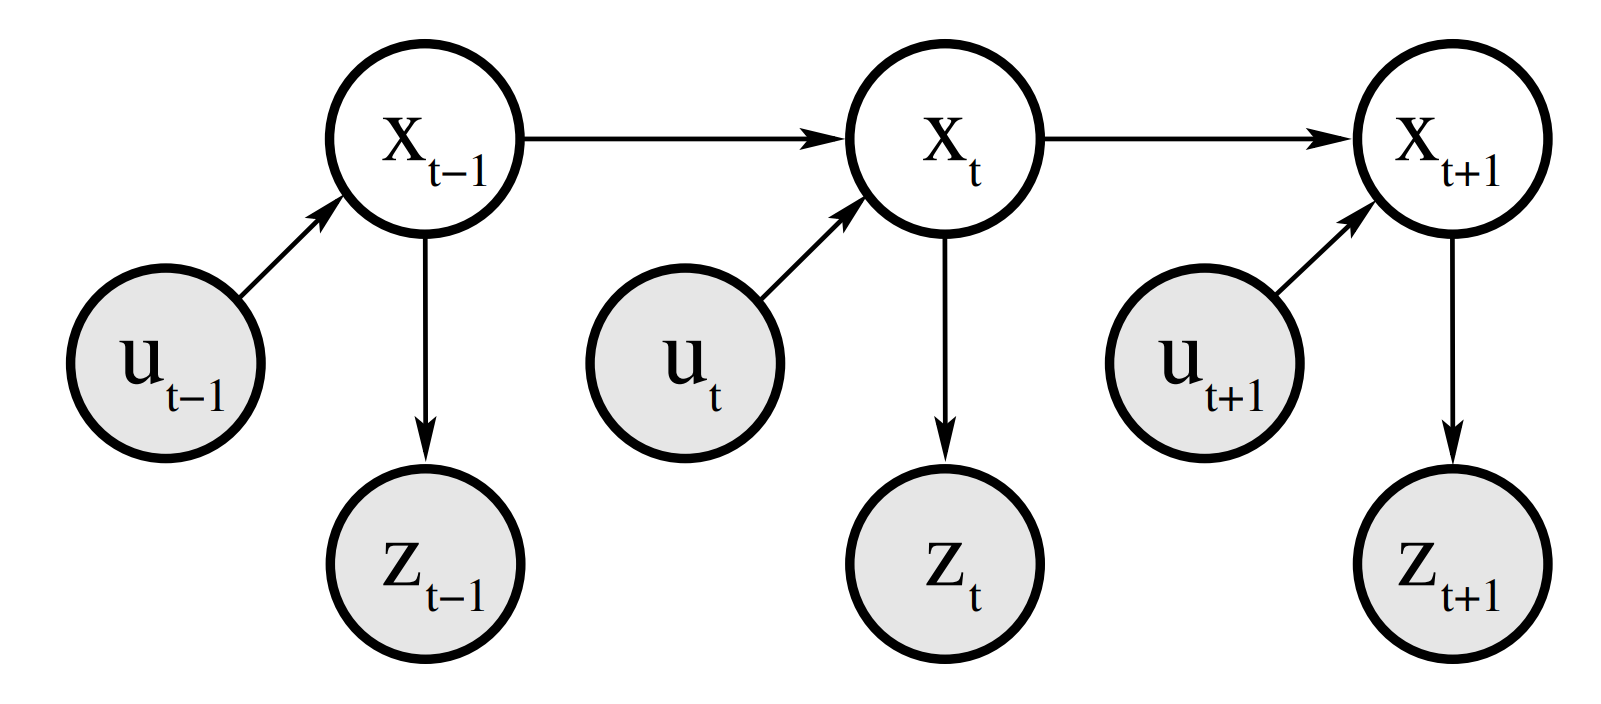
\includegraphics[width=0.8\textwidth]{resources/hidden-markov-model.png}
    \caption{Hubungan $X, U, Z$}
    \label{fig:hidden-markov-model}
\end{figure}

Hubungan ini digambarkan pada gambar \ref{fig:hidden-markov-model}. Peluang yang hanya saling berpengaruh antar tahapan waktu yang berdekatan disebut juga \textit{hidden Markov model} atau \textit{dynamic Bayes network}.

\subsection{Penapis Bayes}

\begin{algorithm}
    \caption{Penapis Bayes}
    \label{alg:bayes-filter}
    \begin{algorithmic}[1]
        \Function{bayes\_filter}{$bel(x_{t-1}), u_t, z_t$}
        \ForAll{$x_t$}
        \State $\overline{bel}(x_t) = \int p(x_t \,|\, u_t, x_{t-1})\, bel(x_{t-1})\, dx_{t-1}$
        \State $bel(x_t) = \eta\, p(z_t \,|\, x_t)\, \overline{bel}(x_t)$ \Comment{$\eta$ menormalisasi nilai dari $bel(x_t)$}
        \EndFor
        \State \Return $bel(x_t)$
        \EndFunction
    \end{algorithmic}
\end{algorithm}

Perhatikan bahwa perubahan nilai dari $\overline{bel}(x_{t-1})$ ke $bel(x_t)$ dapat ditentukan dari peluang transisi keadaan $p(x_t \,|\, x_{t-1}, u_t)$, dan perubahan nilai dari $bel(x_t)$ ke $\overline{bel}(x_t)$ dapat ditentukan dari peluang pengukuran $p(z_t \,|\, x_t)$ menggunakan Teorema Bayes. Memanfaatkan fakta tersebut, dirumuskan algoritma penapis Bayes atau \textit{Bayes filter algorithm} pada algoritma \ref{alg:bayes-filter}. Baris tiga menunjukkan perhitungan nilai $bel(x_t)$ sebagai ekspansi dari penjumlahan nilai $p(x_t, x_{t-1})$ saat diketahui $u_t$ untuk semua kemungkinan $x_{t-1}$, spesifik untuk kasus kontinu. Tahap ini sering disebut tahap prediksi. Baris empat memanfaatkan teorema Bayes untuk mendapatkan distribusi $x_t$ setelah mendapatkan informasi dari $z_t$. Tahap ini sering disebut tahap pembaruan pengukuran.

Algoritma penapis digunakan untuk mengiterasi nilai dari $bel(x_t)$ seiring waktu, dan merupakan algoritma yang optimal mengasumsikan proses merupakan \textit{hidden Markov model}. Perhatikan bahwa algoritma ini mengharuskan pemodelan sendiri nilai dari peluang transisi keadaan, peluang pengukuran, dan distribusi awal $bel(x_0)$ yang akan digunakan.

Selain itu, karena nilai dari $bel(x_t)$ merupakan distribusi peluang, dalam aplikasinya dibutuhkan pendekatan untuk memodelkan distribusi tersebut sehingga dapat dikomputasi oleh komputer. Pada praktisnya, distribusi peluang $bel(x_t)$ dimodelkan sebagai distribusi dengan jenis yang dapat diparameterasikan seperti pada penapis Kalman, atau distribusi tersebut didiskritkan seperti pada penapis histogram atau penapis partikel.

\subsection{Penapis Kalman}

Pada penapis Kalman atau \textit{Kalman Filter} (\textit{KF}), distribusi dari $bel(x_t)$ dan $\overline{bel}(x_t)$ diasumsikan memiliki distribusi Gaussian dengan parameter $\mu$ dan $\sigma^2$ yang dicari pada setiap iterasi algoritmanya. Agar penapis Bayes Gaussian bekerja, distribusi peluang transisi keadaan dan peluang pengukuran harus memiliki restriksi tambahan.

Pada variasi penapis Kalman yang paling sederhana, direstriksi bahwa (1) vektor acak $x_t$ merupakan kombinasi linear dari $x_{t-1}, u_t,$ dan faktor error $\epsilon_t$
\begin{align}
    x_t = A_t x_{t-1} + B_t u_t + \epsilon_t \,
\end{align}
untuk $x_t$ berdimensi $n$, $u_t$ berdimensi $m$, $A_t$ matriks berdimensi $n \times n$, dan $B_t$ berdimensi $n \times m$, dan $\epsilon_t$ vektor acak Gaussian dengan rata-rata nol dan kovariansi $R_t$; (2) $z_t$ merupakan kombinasi linear dari $x_t$ dan faktor error $\delta_t$
\begin{align}
    z_t = C_t x_t + \delta_t
\end{align}
untuk $z_t$ berdimensi $k$, $C_t$ berdimensi $k \times n$, dan $\delta_t$ vektor acak Gaussian dengan rata-rata nol dan kovariansi $Q_t$; dan (3) distribusi awal $bel(x_0)$ memiliki distribusi Gaussian. Ketiga asumsi ini menjamin bahwa distribusi $bel(x_t)$ merupakan distribusi Gaussian untuk semua waktu $t$ yang akan datang.

\begin{algorithm}
    \caption{Penapis Kalman}
    \label{alg:kalman-filter}
    \begin{algorithmic}[1]
        \Function{kalman\_filter}{$\mu_{t-1}, \Sigma_{t-1}, u_t, z_t$}
        \State $\overline{\mu}_t = A_t\, \mu_{t-1} + B_t\, u_t$
        \State $\overline{\Sigma}_t = A_t\, \Sigma_{t-1}\, A_t^T + R_t$
        \State $K_t = \overline{\Sigma}_t\, C_t^T\, (C_t\, \overline{\Sigma}_t\, C_t^T + Q_t)^{-1}$
        \State $\mu_t = \overline{\mu}_t + K_t(z_t - C_t\, \overline{\mu}_t)$
        \State $\Sigma_t = (I - K_t\, C_t)\, \overline{\Sigma}_t$
        \State \Return $\mu_t, \Sigma_t$
        \EndFunction
    \end{algorithmic}
\end{algorithm}

Berdasarkan hubungan di atas, algoritma penapis Kalman menghitung nilai dari parameter rata-rata $\mu_t$ dan kovariansi $\Sigma_t$ dari distribusi Gaussian $bel(x_t)$. Sehingga dapat diturunkan algoritma penapis Kalman seperti pada algoritma \ref{alg:kalman-filter}.

Disebabkan restriksi linearitas pada peluang transisi keadaan dan peluang pengukuran, algoritma penapis Kalman tidak dapat digunakan apabila restriksi linearitas tersebut tidak dipenuhi. Agar penapis Kalman dapat digunakan untuk kasus $x_t = g(u_t, x_{t-1}) + \epsilon_t$ dan $z_t = h(x_t) + \sigma_t$ dimana fungsi $g$ dan $h$ tidak linear, fungsi tersebut harus diaproksimasi terlebih dahulu agar menjadi linear.

Pada \textit{Extended Kalman Filter}, fungsi dilinearkan menggunakan turunan parsial dari fungsi $g$ dan $h$. Dengan menghitung $G_t = g'(u_t, \mu_{t-1})$ dan $H_t = h'(\overline{\mu}_t)$ dimana $g'$ merupakan turunan parsial $g$ terhadap $x_{t-1}$, didapatkan persamaan linear
\begin{align}
    g(u_t, x_{t-1}) \approx g(u_t, \mu_{t-1}) + G_t\, (x_{t-1} - \mu_{t-1}) \\
    h(x_t) \approx h(\overline{\mu}_t) + H_t\, (x_t - \overline{\mu}_t)
\end{align}
Nilai $A$ dan $C$ pada penapis Kalman dapat digantikan dengan nilai $G$ dan $H$.

Pada \textit{Unscented Kalman Filter}, fungsi dilinearkan dengan mengambil sampel nilai pada fungsi $g$ dan $h$, lalu membuat persamaan linear dengan melakukan regresi pada nilai masukan secara umum. Sampel diambil di rata-rata $\mu$ dan dua titik di sekelilingnya untuk setiap dimensi yang ada.

\subsection{Penapis Histogram}

\begin{algorithm}
    \caption{Penapis Bayes Diskrit}
    \label{alg:discrete-bayes-filter}
    \begin{algorithmic}[1]
        \Function{discrete\_bayes\_filter}{$\{p_{k, t-1}\}, u_t, z_t$}
        \ForAll{$k$}
        \State $\overline{p}_{k, t} = \sum_i p(X_t = x_k \,|\, u_t, X_{t-1} = x_i)\, p_{i, t-1}$
        \State $p_{k, t} = \eta\, p(z_t \,|\, X_t = x_k)\, \overline{p}_{k, t}$ \Comment{dinormalisasi untuk semua $k$}
        \EndFor
        \State \Return $\{p_{k, t}\}$
        \EndFunction
    \end{algorithmic}
\end{algorithm}

Pada penapis histogram, kemungkinan nilai dari $x_t$ terbatas dan dibagi-bagi menjadi sebanyak terbatas daerah, misalnya kemungkinan posisi dari robot pada lapangan berdimensi $9 \times 6$ meter persegi dapat dibagi menjadi $1350$ daerah berbentuk persegi berukuran $20 \times 20$ sentimeter persegi dalam suatu grid. Pada algoritma ini, $bel(x_t)$ direpresentasikan sebagai suatu tabel yang menyimpan peluang nilai berada dalam masing-masing daerah yang ada. Algoritma ini pun relatif lebih sederhana karena hanya perlu mendiskritkan perhitungan pada filter Bayes.

Algoritma filter Bayes diskrit ada di algoritma \ref{alg:discrete-bayes-filter}. Apabila fungsi peluang transisi keadaan atau peluang pengukuran yang dimiliki bersifat kontinu, dapat diaproksimasi menjadi diskrit seperti
\begin{align}
    p(\mathbf{x}_{k, t} \,|\, u_t, \mathbf{x}_{i, t-1}) \approx |\mathbf{x}_{k, t}|\, p(\hat{x}_{k, t} \,|\, u_t, \hat{x}_{i, t-1}) \\
    p(z_t \,|\, \mathbf{x}_{k, t}) \approx p(z_t \,|\, \hat{x}_{k, t})
\end{align}
dimana $\hat{x}_{k, t}$ adalah representasi dari daerah $\mathbf{x}_{k, t}$ seperti titik tengahnya, dan $|\mathbf{x}_{k, t}|$ adalah luas daerahnya

Teknik histogram ini berkaitan erat dengan grid okupansi dimana masing-masing daerah di grid tersebut diisi dengan tingkat kepercayaan suatu nilai berada dalam daerah tersebut, walau berbeda dengan histogram peluang dimana jumlah dari nilai semua grid haruslah bernilai satu. Aplikasi dari teknik ini dalam permasalahan lokalisasi robot kerap disebut dengan \textit{Markov localization}.

\subsection{Penapis Partikel}

Pada penapis partikel, distribusi peluang nilai dari $bel(x_t)$ direpresentasikan dengan menyimpan koleksi sejumlah nilai $x_t$ atau disebut sebagai partikel, dimana distribusi dari partikel tersebut mengaproksimasi distribusi dari $bel(x_t)$ yang sesungguhnya. Semakin banyak partikel yang disimpan, semakin akurat algoritma penapis partikel ini, tetapi semakin besar juga sumber daya memori dan waktu yang dibutuhkan.

\begin{algorithm}
    \caption{Penapis Partikel}
    \label{alg:particle-filter}
    \begin{algorithmic}[1]
        \Function{particle\_filter}{$\chi_{t-1}, u_t, z_t$}
        \State $\overline{\chi}_t= \overline{\chi}_t = \emptyset$
        \For{$m = 1$ to $M$}
        \State sample $x_t^{[m]} \sim p(x_t \,|\, u_t, x_{t-1}^{[m]})$
        \State $w_t^{[m]} = p(z_t \,|\, x_t^{[m]})$
        \State add $(x_t^{[m]}, w_t^{[m]})$ to $\overline{\chi}_t$
        \EndFor
        \For{$m = 1$ to $M$}
        \State draw $i$ with probability $\propto w_t^{[i]}$
        \State add $x_t^{[i]}$ to $\chi_t$
        \EndFor
        \State \Return $\chi_t$
        \EndFunction
    \end{algorithmic}
\end{algorithm}

Algoritma penapis partikel digambarkan di algoritma \ref{alg:particle-filter}. Baris empat merupakan tahap prediksi dimana untuk setiap partikel sebelumnya dibangkitkan partikel sekarang menggunakan nilai kontrol. Partikel tersebut disimpan di himpunan $\overline{\chi}_t$ beserta evaluasi peluangnya berdasarkan pengukuran. Agar suatu partikel dengan peluang yang lebih besar memiliki lebih banyak representasi dalam himpunan $\chi_t$, dilakukan sampling ulang terhadap $x_t$ dengan peluang sebanding dengan hasil evaluasinya, pada baris delapan sampai sebelas.

Secara umum, penapis partikel ini merupakan pilihan paling populer dalam melakukan estimasi terhadap keadaan nonGaussian, karena komputasinya yang mengandalkan sampling relatif lebih mudah dan tingkat akurasi terhadap performa algoritma dapat diatur dengan mudah melalui banyak partikel yang digunakan. Ada beberapa kondisi yang mengakibatkan ketidakakuratan pada algoritma ini, seperti saat terjadi konvergensi partikel di nilai yang salah, sehingga peningkatan pada algoritma ini diantaranya adalah dengan menambahkan faktor error tambahan pada tahap prediksi dan/atau memasukkan partikel baru di luar $\overline{\chi}_t$ ke dalam $\chi_t$.

Penggunaan populer dari algoritma ini adalah pada algoritma \textit{Monte Carlo localization} (\textit{MCL}) dimana penapis partikel digunakan untuk kasus lokalisasi robot menggunakan data kontrol dari kontrol kecepatan atau data perpindahan dari sensor dan data pengukuran dari sensor peraba jarak atau kamera. Algoritma \textit{Augmented Monte Carlo localization} (\textit{AMCL}) merupakan modifikasi algoritma \textit{MCL} biasa yang ditambahkan pemasukkan partikel baru apabila hasil evaluasi partikel-partikel yang ada sekarang lebih buruk dari sebelumnya.

\section{Studi Terkait}

Secara umum, teknik probabilistik seperti penapis Kalman maupun penapis partikel telah banyak diimplementasi dalam kasus pelacakan objek oleh satu agen dan telah menunjukkan tingkat keberhasilan yang cukup baik. Sedangkan dalam kasus pelacakan objek oleh banyak agen, terdapat banyak studi yang mencetuskan beragam ide yang sangat bervariasi dalam berbagai konteks. Dalam konteks kontes robot sepak bola sendiri, sudah terdapat beberapa studi yang mencoba menggabungkan data pelacakan objek maupun lokalisasi.

Robot-robot \cite{stroupe2001} melacak posisi bola menggunakan penapis Kalman dan distribusi hasilnya disebarkan ke robot lainnya, dimana distribusi Gaussian dari semua robot akan digabungkan oleh masing-masing robot untuk menghasilkan suatu distribusi Gaussian akhir. Asumsi dasar dari makalah ini adalah \textit{error}nya bersifat normal independen, lokalisasi robot sempurna, dan waktu pengukuran bersamaan.

\cite{ferrein2005} membandingkan beberapa metode untuk menggabungkan observasi bola dari masing-masing robot, seperti merata-ratakan posisi pengamatan, menggunakan penapis Kalman menggunakan terhadap posisi bola menggunakan data yang didapat masing-masing robot, menggunakan penapis partikel, maupun menggunakan penapis histogram yang digabungkan ke estimasi global menggunakan penapis Kalman. Hasilnya adalah penapis Kalman sederhana memiliki tingkat akurasi dan kecepatan yang paling baik.

Masing-masing robot \cite{pahliani2006} melakukan lokalisasi menggunakan \textit{Markov localization}, lalu tergantung dari posisi robot, robot-robot yang ada membentuk beberapa kelompok kecil untuk bertukar informasi. Data dari robot di kelompok yang sama dibagikan, lalu menggunakan data yang didapat dari kelompok lain, hasil lokalisasi dari masing-masing robot diperbaiki secara Bayes. Setelah lokalisasi, deteksi objek juga dilakukan menggunakan alur dan kelompok yang sama.

\cite{santos2009} melacak bola menggunakan penapis partikel. Untuk mengefisiensikan pertukaran informasi antar robot, distribusi dalam bentuk partikel diubah dulu menjadi \textit{gaussian mixture model} yang terdiri dari beberapa distribusi Gauss menggunakan algoritma \textit{expectation maximization} yang bekerja mirip seperti algoritma \textit{K means}. Ada juga ukuran persetujuan informasi antar robot menggunakan \textit{covariance intersection} untuk menentukan apakah informasi baru diintegrasi dengan informasi robot sendiri atau tidak. \cite{ahmad2011} mengembangkan ide ini dengan membuat algoritma penggabungan distribusi dari masing-masing robot dimana dibangkitkan kumpulan partikel baru dengan melakukan \textit{sampling} dari distribusi-distribusi yang ada berdasarkan tingkat kepercayaan distribusi tersebut sebagai masukan dari penapis partikel.

\cite{ahmad2013} mengumpulkan semua pengukuran posisi relatif semua robot terhadap robot lain, objek statis, maupun objek dinamis, dan mencari konfigurasi posisi semua objek yang meminimasi \textit{error} dari pengukuran-pengukuyan yang ada menggunakan \textit{iterative local linearization} atau \textit{least square minimzation}. Kelebihan teknik ini diantara adalah beban komputasinya linear terhadap banyak robot, akan tetapi setiap robot harus menunggu sampainya data pengukuran dari semua robot lain.

\cite{chang2016} menggunakan \textit{Extended Kalman Filter} untuk melacak sistem seluruh robot dan objek. \textit{Update} dilakukan untuk masing-masing robot, sedangkan pengukuran diintegrasi berdasarkan robot apa saja yang terlibat dalam pengukuran tersebut. Teknik \textit{multiple hypothesis tracking} digunakan untuk mengasosiasikan data pengukuran dengan posisi objek di hipotesis.

\cite{ahmad2017} menggunakan penapis partikel yang mencakup posisi semua robot ditambah objek yang diobservasi. Masing-masing bagian partikel dari robot digerakan dan dievaluasi secara terpisah, dan diurutkan ulang sehingga bagian partikel dengan evaluasi tinggi dari suatu robot dipasangkan dengan bagian partikel robot lain dengan evaluasi yang tinggi juga. Algoritma ini lalu memasangkan partikel bagian dari objek yang memaksimalkan evaluasi partikel bagian tersebut dengan partikel bagian robot dengan evaluasi tinggi juga. Teknik ini menyelesaikan masalah defisiensi partikel pada penapis partikel tanpa harus menambahkan banyak partikel secara eksponensial.


\chapter{ANALISIS DAN PERANCANGAN}

\section{Analisis Masalah}

Hampir semua studi pengembangan algoritma estimasi \textit{world model} yang melacak posisi robot maupun bola di kontes robot sepak bola mengasumsikan bahwa komunikasi antar robot memiliki latensi yang dapat diabaikan dan belum ada yang mencoba menangani secara eksplisit dan menganalisis pengintegrasian data dari robot lain yang terlambat. Secara umum, masih sedikit studi yang membahas penggabungan data pengukuran sensor dengan latensi pada sistem komputasi terdesentralisasi.

\section{Lingkungan Implementasi}

\begin{figure}[h]
    \centering
    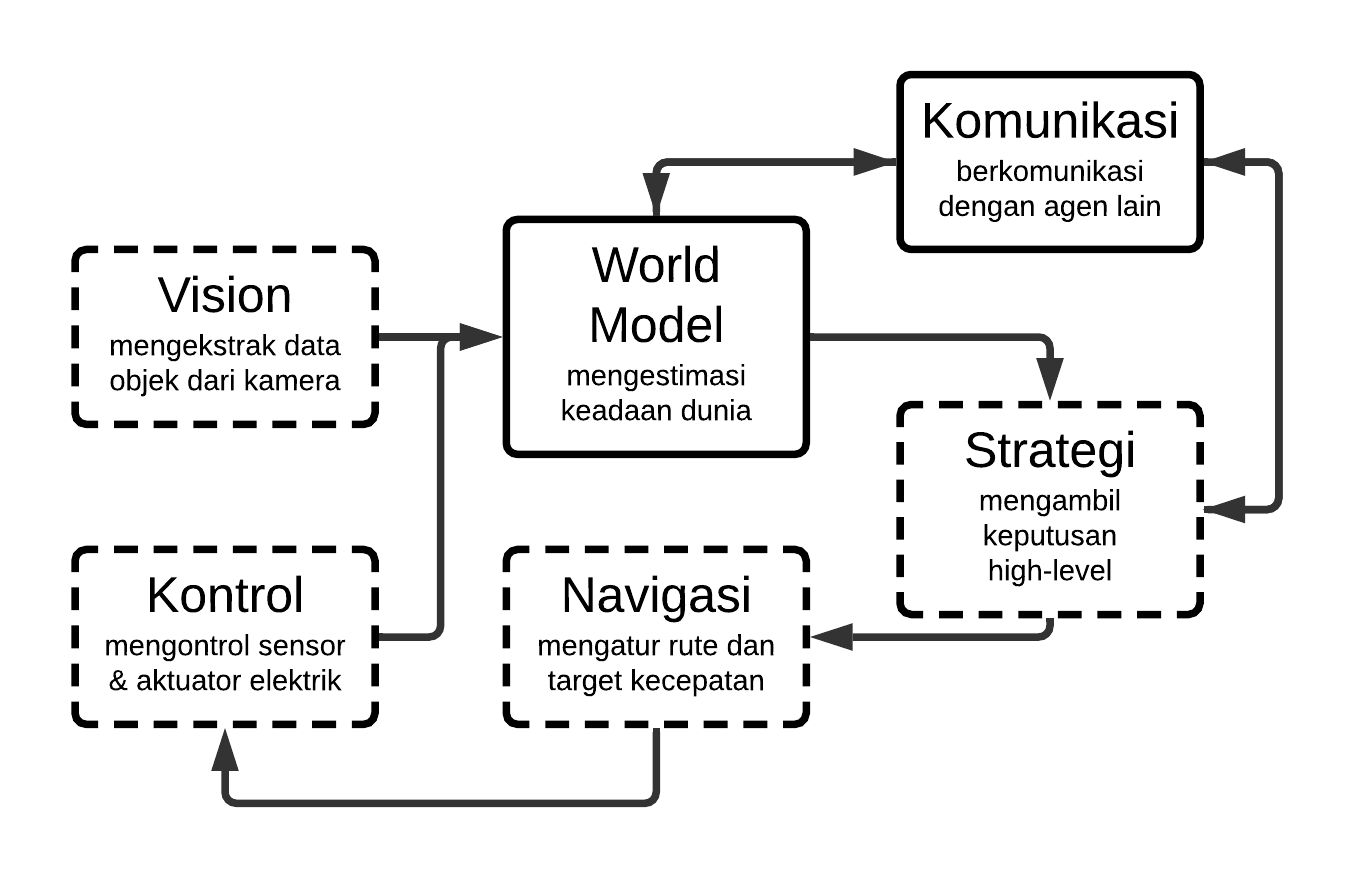
\includegraphics[width=0.8\textwidth]{resources/dagozilla-structure.png}
    \caption{Struktur modul Dagozilla}
    \label{fig:dagozilla-structure}
\end{figure}

Lingkungan perangkat lunak DAGOZILLA menggunakan \textit{platform} \textit{Robot Operating System} (\textit{ROS}) yang memungkinkan komunikasi antar proses oleh modul-modul aplikasi yang menjalankan fungsi-fungsi robot menggunakan paradigma \textit{publish-subscribe} pesan atau \textit{request-response} \textit{service} yang disediakan suatu modul. Modul-modul yang ada digambarkan pada gambar \ref{fig:dagozilla-structure}.

Fokus utama dari tugas akhir ini adalah mengembangkan modul \textit{world model} yang bertugas untuk memproses semua data persepsi dari modul sebelumnya maupun informasi dari robot lain untuk menyediakan estimasi keadaan dunia yang seakurat dan sefaktual mungkin agar dapat digunakan dalam melakukan pengambilan keputusan.

Modul kontrol berkomunikasi dengan mikrokontroler yang berhubungan langsung dengan \textit{hardware} untuk mengontrol aktuator dan mengambil data dari sensor-sensor lokal, diantaranya odometri motor penggerak dan kompas. Odometri mengukur perputaran yang dilakukan masing-masing roda penggerak yang dapat diolah menjadi data perpindahan dan kompas mengukur orientasi global dari robot itu sendiri.

Modul \textit{vision} mengekstrak data dari kamera, diantaranya posisi bola dari gambar menggunakan deteksi warna dan momen objek, dan sebaran titik dari garis lapangan maupun objek penghalang lapangan menggunakan algoritma \textit{radial search line}.

\section{Analisis dan Desain Umum Solusi}

Sebagai gambaran besar hipotesis solusi, masing-masing robot tetap harus melakukan estimasi sendiri menggunakan data yang tersedia dari sensor lokal robot tersebut. Hal ini dilakukan agar masing-masing robot harus tetap memiliki estimasi informasi krusial seperti posisi robot sendiri, bola, ataupun penghalang walaupun terjadi kegagalan jaringan komunikasi. Algoritma secara umum harus berjalan secara \textit{online} tanpa masing-masing robot harus menunggu informasi dari robot lain terlebih dahulu sebelum dapat dijalankan. Penapis partikel dianggap sebagai metode yang cukup baik untuk melacak posisi robot maupun bola yang dapat bergerak secara bebas.

Masing-masing robot lalu menyiarkan hasil pemrosesan lokalnya ke semua robot lain. Mengirimkan keseluruhan informasi pengukuran secara mentah dianggap kurang dapat diandalkan dan meningkatkan beban komputasi untuk semua robot melihat ada data seperti persepsi garis lapangan dan objek penghalang yang terdiri dari puluhan sampai ratusan data titik. Data seperti sebaran partikel estimasi haruslah diproses dahulu ke bentuk lain seperti \textit{Gaussian Mixture Model} sebelum disiarkan ke robot lain.

Data yang disiarkan mengandung \textit{time-stamp} pengolahan data agar robot yang menerima dapat mendeteksi dan melakukan pengolahan tambahan untuk data yang terlambat. Data juga mengandung ukuran tingkat kepercayaan keakuratan yang ditetapkan robot penyiar. Hal ini dilakukan karena walaupun pertukaran informasi dapat meningkatkan akurasi, hal tersebut juga dapat menyebabkan penyebaran \textit{error} dalam estimasi, sehingga harus didesain sehingga informasi dengan tingkat kepercayaan yang rendah tidak terlalu mempengaruhi informasi dengan tingkat kepercayaan yang lebih tinggi.

Diagram alir hipotesis solusi digambarkan di \ref{fig:solution-flowchart}.

\begin{figure}[h]
    \centering
    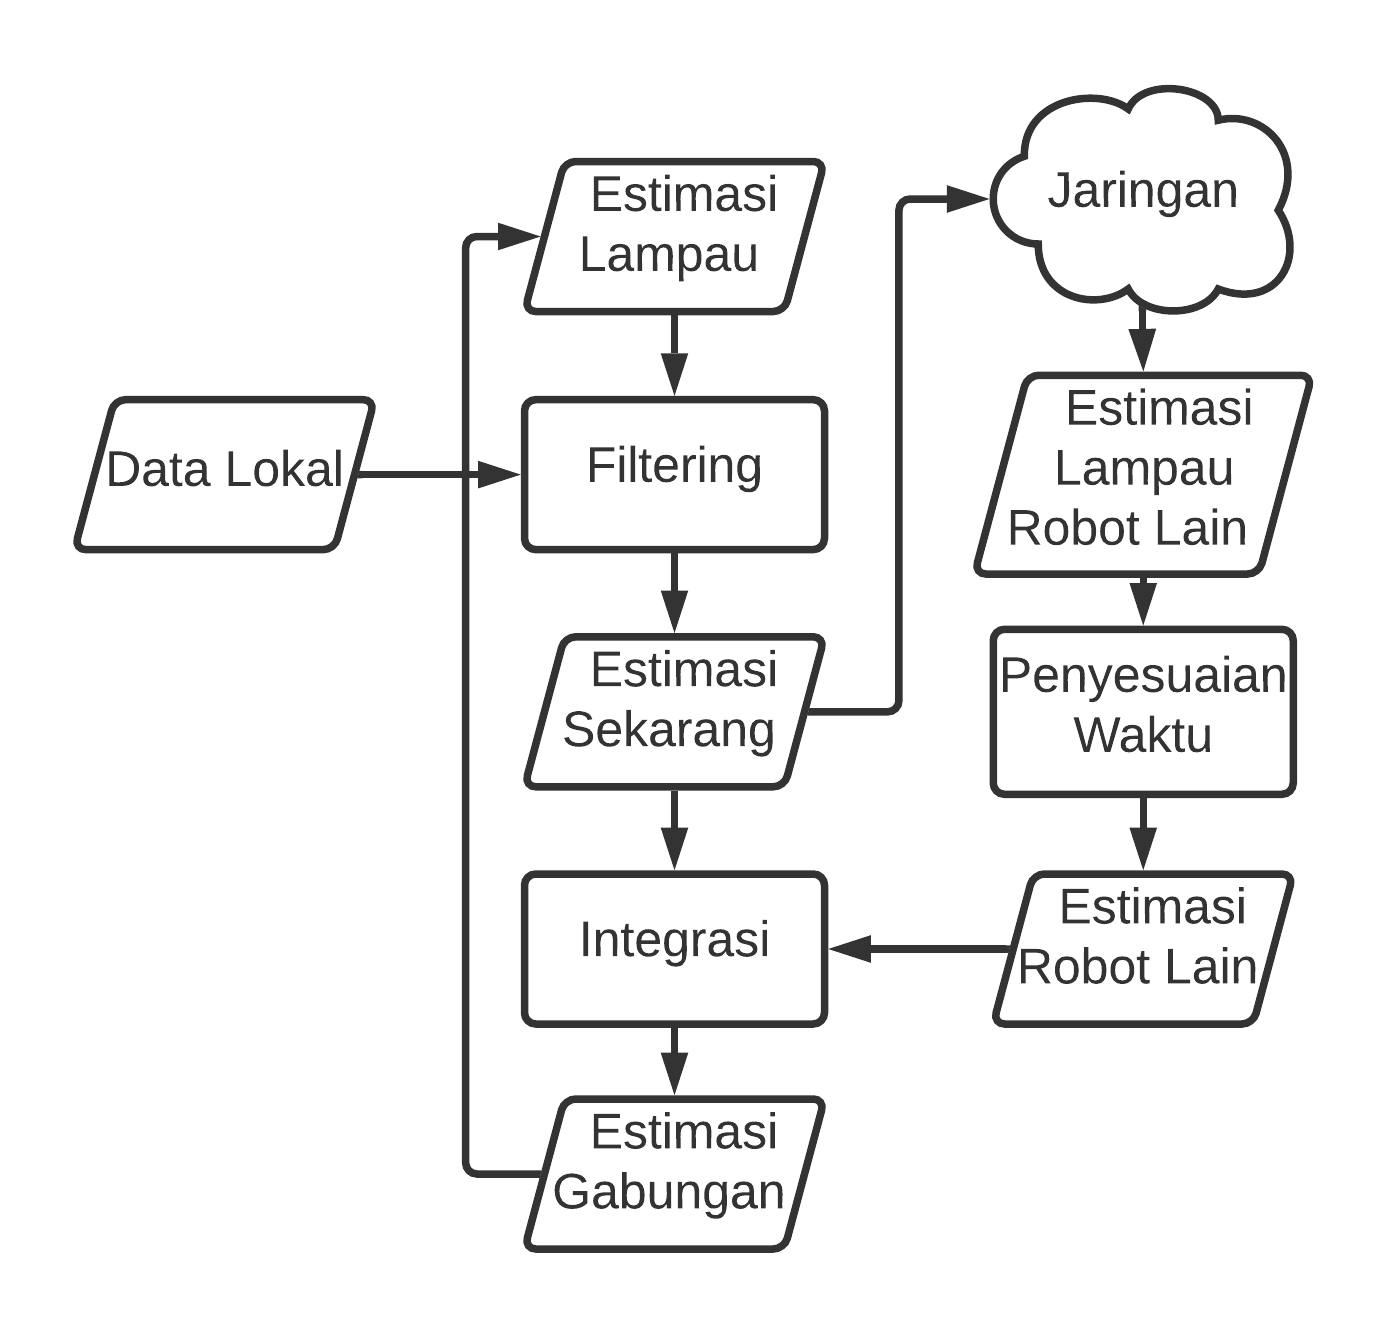
\includegraphics[width=0.8\textwidth]{resources/solution-flowchart.png}
    \caption{Diagram alir hipotesis solusi}
    \label{fig:solution-flowchart}
\end{figure}
% \input{chapters/chapter-4}
% \input{chapters/chapter-5}
%----------------------------------------------------------------%

\begingroup
\renewcommand{\baselinestretch}{1.0}
\printbibliography[heading=bibintoc]
\endgroup

% Format judul bab lampiran
% \titleformat{\chapter}[hang]
%   {\large\bfseries}
%   {\chaptertitlename\ \thechapter}{1em}
%     {\large\bfseries}
% \titlespacing*{\chapter}{0pt}{-1.5\baselineskip}{\parskip}

% \begin{appendices}
%     \input{chapters/appendix-1}
%     \input{chapters/appendix-2}
% \end{appendices}

\end{document}